\chapter{Task1}

	We have to find the Top 50 Locality Places (City) based on Number of Photos taken at that location. Photos taken in Neighbourhood Places within that locality has to be considered for that place itself. For each of those top 50 places we need to find the top 10 tags which has most number of photos tagged with it.
		
\section{Design}
	We have created 3 Jobs for solving the problem chained one after another \\
	\begin{itemize}
		\item [Job1:] creates counts the photos per locality  
		\item [Job2:] Sorts and Give Top 50 Locality 
		\item [Job3:] For the Top 50 Locality, Finds the top 10 tags 
	\end{itemize}

	
	\emph{Design Choice 1:}  Use of Distributed Cache \\
		Since the current number of places has about 300,000 Entries and the size is about 33 MB, we have decided to use it as a distributed cache rather than running a Mapreduce job for joining the places and photos. If each Hash entry takes about 128 Bytes (Hash, String, Value) then for a million entry it would be 128 MB. Given the RAM capacity of modern machine, this approach can scale easily upto 8 Million Entries for 1G of RAM and even more. \\
		\\
	\emph{Design Choice 2:} Reading the Photos Data Twice \\
	 	We implemented a map which reads the data and spits out two types output. One for tags and other for unique users. With that implementation the data output was about 20 Gigabytes. For the 80 Million entries for photos there we 700 million tags. Due to that we had huge amount of data which are useless causing lot of time in shuffling. And most of the data is useless as we are only concerned about top 50 locations. So we read the data again but only output tags for top 50 locations. This reduced timings massively.
	 	
	 	It also fails to scale, if your data goes into peta bytes the output generated will be 10x peta bytes which will be impossible to even store. So Reading the data twice is the right option.

	Due to these optimisations, we could get the total Running time for the problem is ~ 5 Minutes.
	
	Our design is scalable because
	\begin{enumerate}
	\item We have used Combiner everywhere to make sure less shuffling 
	\item Since we output tags only for top 50 we can scale to Petabytes still we get the best performance
	\item We use Framework to sort for better and efficient sorting	
	\end{enumerate}

\subsubsection{Job1}

\small
\begin{tabular}{| c | p{2cm} | p{2cm} | p{7cm} | }
\hline 
 Segments 
 & Input 
 & Output 
 & Pseudocode \\ \hline
 
 Mapper 
 & \scriptsize 
 1. Cache: Place.txt \newline
 2. Photos Data
 & \scriptsize 
Key: PlaceName \newline
Value: 1
 & \scriptsize 
 Setup: \newline
 1. create HashMap with (key, value) as (placeid, Placename) \newline
 2. For each line in Place.txt \newline
 		HashMap[placeid] = Placename \newline
 Map: \newline
 2. For each Text Input \newline
 		placename = HashMap(placeid)\newline
 		output(placename, 1) \newline
 \\ \hline
 
 Combiner 
 & \scriptsize
Key: PlaceName \newline
Value: 1

 & \scriptsize 
Key: PlaceName \newline
Value: List(1)
 & \scriptsize 
 Foreach  in List(1): \newline
 	 count = count + 1 \newline
 output(Placename, count) \newline
  \\ \hline
 
  Reducer 
 & \scriptsize 
Key: Place Name \newline
Value: List(count) \newline
 & \scriptsize 
Key: Place Name \newline
Value: numPhotos \newline
 & \scriptsize 
 Foreach count in List(count): \newline
 	 numPhotos = numPhotos + count \newline
 output(Placename, numPhotos) \newline
 \\ \hline
 
\end{tabular}


\subsubsection{Job2}


\small
\begin{tabular}{| c | p{3cm} | p{3cm} | p{5cm} | }
\hline 
 Segments 
 & Input 
 & Output 
 & Comments \\ \hline
 
 Mapper 
 & \scriptsize
Key: placename \newline
Value: numPhotos \newline
 & \scriptsize 
Key: numPhotos \newline
Value: Placename \newline
& \scriptsize
For Each Key, Value \newline
	output(Value, Key) \newline
 \\ \hline
 
Sorter 
& \multicolumn{2}{ |c| }{ Sort in Reverse Order }
& \scriptsize Extend Writablecomparable to reverse sort the integer and pass it to the driver. 
  \\ \hline
 
  Reducer 
 & \scriptsize 
Key: numPhotos \newline
Value: Place Name \newline
 & \scriptsize 
Key: Place Name \newline
Value:  numPhotos \newline
 & \scriptsize 
For first 50: Key and Value \newline
	Output(value, key) \newline
 \\ \hline
\end{tabular}


\subsubsection{Job3}
	We implemented the Job3 into two different jobs one which counts and other sorts and the perfomance was worse than the current implementation. 
		
	We find it unnecessary because the scale of data which is very minimal. Below is the statistics for the given data \newline
	Total Tags = 700 Million \newline
	Top 50 Location Tags = 140 Million\newline
	After combiner = 13 Million\newline
	Total Groups = 5 Million\newline
	We can have as much as 50 Reducers to parallelize \newline
	Reducer Load = 0.1 Million  \newline

	Block Size of 128 MB ~= 	10 Million Groups\newline
	This job should be able to process data in Tera Byte scale easily.  \newline

\bgroup
\scriptsize
\begin{tabular}{| c | p{3cm} | p{3cm} | p{5cm} | }
\hline 
 \textbf{Segments}
 & \textbf{Input}
 & \textbf{Output} 
 & \textbf{Pseudocode} \\ \hline
 
 Mapper 
 & 
 Cache1: Place.txt
 Cache2: Top 50 Places
 & 
Key: (PlaceName, Tag)
Value: 1
& 
 \textbf{Setup:} \newline
 1. create HashMap with (key, value) as (placeid, Placename) \newline
 2. For each line in Place.txt \newline
 		HashMap[placeid] = Placename \newline
\textbf{Map} \newline
1. For each Photo: \newline
	if Place is in Top 50 Places then \newline
		Output( (PlaceName, Tag), 1) \newline
 \\ \hline

 Combiner 
 & 
Key: (PlaceName, Tag)
Value: 1
 & 
Key: (PlaceName, Tag)
Value: (tagcount)
& 
 Foreach count in List(count): \newline
 	 tagcount = tagcount + count \newline
 Output( (PlaceName,Tag), tagcount) \newline
 \\ \hline 
 
 Partitioner 
&
\multicolumn{3}{ |c| }{ Partition based on Place Name} \\
  \\ \hline

  Reducer 
 & 
Key: (PlaceName, Tag)
Value: (tagcount)
 & 
 PlaceName \t numberOfPhotos \t (tag:freq)+
 & 
 \textbf{Reduce:} \newline
 For each key, List(tagcount): \newline
 	totaltagcount = totaltagcount + tagcount \newline
  If totaltagcount > one of top 10 tags for the place \newline
 	add to top 10 tags \newline
 else \newline
 	ignore tags \newline
 	
 \textbf{cleanup:} \newline
 	For each place: \newline
 		output(PlaceName \t numberOfPhotos \t (tag:freq)+) \newline

 \\ \hline
\end{tabular}
\egroup

\section{Performance}

For a highly scalable Map Reduce Job we need to make sure the following parameters are minimized
	\begin{enumerate}
	\item Time Taken for a  Map Task
	\item Time Taken for Shuffling
	\item Time Taken for a Reduce Task
	\end{enumerate}
	
	Higher the number of shuffle bytes, more the time for reduce task. So knowing where the time is more gives us better idea to optimize the solutions.	
	
	Below is our performance graph for our implementation. On X-Axis is the Input Size and on Y-Axis is Total Time taken by all mapper or Reducer. We have plotted both Mapper, Reducer, Mapper + Reducer. Due to our design the amount of work done in reducer is very minimal. 
	
	The overall running time is less than 5 Minutes, given we have enough Mapper task to run in parallel. 
	
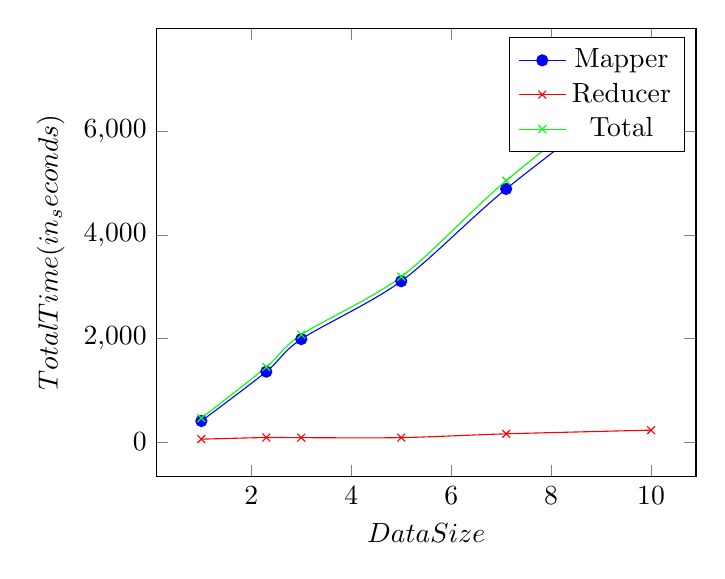
\begin{tikzpicture}
    \begin{axis}[
        xlabel=$DataSize$,
        ylabel=$TotalTime(in_seconds)$]
    \addplot[smooth,mark=*,blue] plot coordinates {
        (10, 7035)
        (7.1,4885)
        (5,3104)
        (3, 1987)
        (2.3,1359)
        (1.0, 406)
    };
    \addlegendentry{Mapper}

    \addplot[smooth,color=red,mark=x]
        plot coordinates {
            (10,230)
            (7.1,159)
            (5, 86)
            (3, 85)            
            (2.3,88)
            (1.0,56)
        };
		\addlegendentry{Reducer}
		
	    \addplot[smooth,color=green,mark=x]
        plot coordinates {
            (10,7265)
            (7.1,5044)
            (5, 3190)
            (3, 2072)            
            (2.3,1447)
            (1.0,462)
        };    
    
    	\addlegendentry{Total}
    \end{axis}
    \end{tikzpicture}
    